\section{Methodik}\label{sec:methodik}
\subsection{Beschreibung der Algorithmen}
StudyMap soll Studieninteressierten einen schnellen Überblick über
alle in Frage kommenden Studiengänge ermöglichen.  Dabei soll dem Nutzer eine
interaktive Grafik präsentiert werden, mit der er anhand von Studieninhalten
(z.B. \glqq Gesundheit und Soziales\grqq{}) sofort alle relevanten Studiengänge
findet. Dazu ist es notwendig, die Studiengänge nach ihren Inhalten zu
gruppieren (Clustering) und schließlich visuell ästhetisch aufzubereiten.

Bei der Festlegung des Clustering-Algorithmus für den Studiengangsfinder wurden
verschiedene Optionen in Betracht gezogen, darunter K-Means Clustering,
Force-Directed Layouts und Multidimensionale Skalierung. Nach einer
gründlichen Abwägung der Vor- und Nachteile fiel die Wahl auf MDS. Die Gründe
für diese Entscheidung und eine Erläuterung der jeweiligen Algorithmen werden in
den folgenden Kapiteln gegeben.

\subsubsection{Force-Directed-Graphs}
Force-Directed Graph Drawing ist eine Methode zur Visualisierung von Graphen, bei der die Positionen der Knoten und Kanten aufgrund von Kräften bestimmt werden. Das Vorgehen hierbei ist vereinfacht inspiriert von Modellen der Teilchenphysik und wird häufig mit dem Verhalten von Federn verglichen. Ziel des Algorithmus ist es durch Kanten verbundene Knoten nah beinander zu platzieren und somit eine ästhetisch ansprechende Visualisierung eines Graphen zu berechnen. In \autoref{fig:force-directed-layouts} erkennt man ausgehend von einer zufälligen Positionierung (Zustand 0), eine schrittweise Optimierung der Darstellung. Wie stark oder schwach sich die Knoten jeweils \glqq anziehen\grqq{} bzw. \glqq abstoßen\grqq{} wird durch die Gleichmäßigkeit der Verteilung auf der Zeichenfläche, auch Canvas genannt, bestimmt. \parencite{schonfeld_fruchtermanreingold_2019}

\begin{figure}[H]
    \centering
    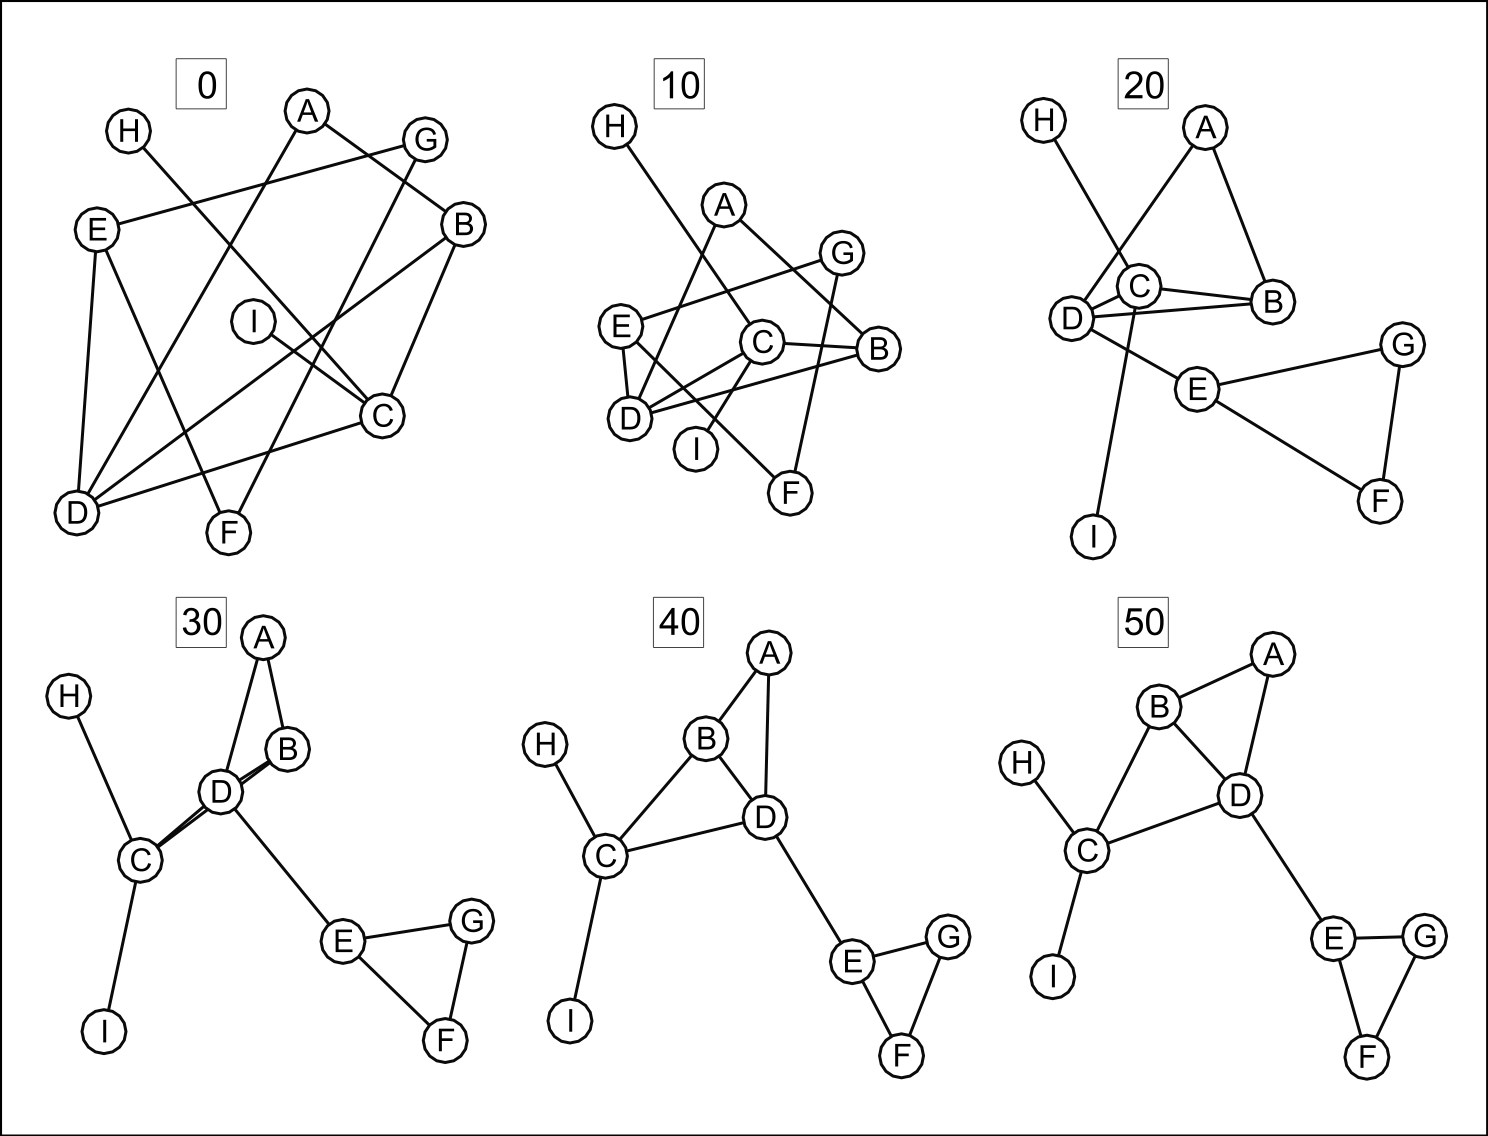
\includegraphics[width=\textwidth]{force-directed-layouts}
    \caption{Schrittweises Durchführen des Layout-Algorithmus von Fruchterman/Reingold}
    \bildquelle{Fruchterman, Thomas M. J./Reingold, Edward M.: Graph Drawing by Force-Directed Placement}
    \label{fig:force-directed-layouts}
\end{figure}

Force-Directed Layouts sind besonders effektiv für die übersichtliche
Darstellung von Netzwerken, in denen die Verbindungen zwischen den Elementen im
Vordergrund stehen. \parencite{schonfeld_fruchtermanreingold_2019} Im Gegensatz dazu
erfordert der Studiengangsfinder eine kontinuierliche Positionierung der
Studiengänge basierend auf inhaltlichen Ähnlichkeiten, was nicht unbedingt der
Stärke von Force-Directed Layouts entspricht. Force-Directed Graph Drawing
benötigt als Vorraussetzung bereits einen Graphen mit Knoten und Kanten, welche
im Fall des Studiengangsfinders die Ähnlichkeiten zwischen den einzelnen
Studiengängen entsprechen würde. Gerade die Berechnung der Ähnlichkeit zwischen
den einzelnen Studiengängen ist jedoch wesentlicher Bestandteil dieser Arbeit,
weshalb der Algorithmus nicht näher untersucht wurde.

\subsubsection{K-Means Clustering Algorithmus}
K-Means ist ein Clustering-Algorithmus, der Datenpunkte in $k$ vordefinierte
Gruppen oder Cluster einteilt. Die Wahl von $k$ stellt die Anzahl der Cluster dar,
und der Algorithmus versucht, die Datenpunkte so zu gruppieren, dass die Varianz
innerhalb der Cluster minimiert wird (siehe \autoref{fig:kmeans}).
\parencite{jeffares_k-means_2019}

\begin{figure}[H]
    \centering
    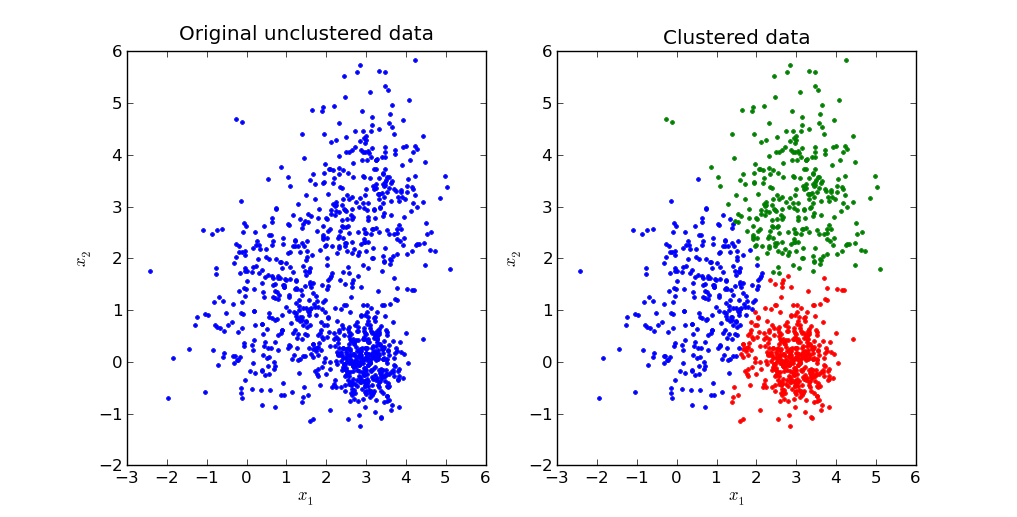
\includegraphics[width=\textwidth]{kmeans}
    \caption{K-Means Clustering Algorithmus}
    \bildquelle{https://mubaris.com/posts/kmeans-clustering/}
    \label{fig:kmeans}
\end{figure}

Die Entscheidung, den K-Means-Algorithmus nicht zu verwenden, basiert darauf, dass dieser hauptsächlich darauf abzielt, Datenpunkte zu gruppieren und weniger auf deren präzise Positionierung in einem zweidimensionalen Raum. Der Algorithmus fordert außerdem eine vordefinierte Clusteranzahl $k$. Das stellt im Falle des Studiengangsfinders jedoch keine Einschränkung dar, da jeder Cluster eine Inhaltskategorie, wie zum Beispiel \glqq Informatik\grqq{} repräsentieren würde. Dennoch ist der K-Means-Clustering-Algorithmus aufgrund seiner Empfindlichkeit gegenüber Ausreißern ungeeignet. Der Algorithmus versucht, Clusterzentren zu finden, die die Gesamtvarianz minimieren. Wenn es Ausreißer in den Studienschwerpunkten gibt, könnten sie das Ergebnis beeinflussen. \parencite{roth_demonstration_2023}

\subsubsection{Multidimensionale Skalierung (MDS)}\label{sec:MDS}
MDS ermöglicht die Reduktion $n$-dimensionaler Daten auf $m$-Dimensionen,
wodurch eine anschauliche Darstellung in Form von Koordinatenpaaren
ermöglicht wird \parencite{intro-to-multidimensional-scaling}. Dieser Aspekt ist
entscheidend, um Studiengänge in einem zweidimensionalen Diagramm zu
positionieren, wobei ähnliche Studiengänge aufgrund ihrer inhaltlichen
Ähnlichkeiten nahe beieinander liegen. Die Anwendung des MDS-Algorithmus auf
eine genormte Tabelle, in der im Falle von StudyMap die Studiengänge nach ihren
Anteilen an verschiedenen Inhaltskategorien gewichtet sind, ermöglicht eine
effektive Positionierung im Diagramm (siehe \autoref{table:input-mds}).

\begin{table}[!ht]
    \centering
    \begin{tabular}{|l|l|l|l|l|l|l|}
    \hline
        \textbf{Kürzel} & \textbf{Architektur} & \textbf{Gesundheit} & \textbf{Technik} & \textbf{Informatik} & \textbf{Wirtschaft} & \textbf{Internat.} \\ \hline
        \textbf{AT} & 0,55 & 0,06 & 0,09 & 0,04 & 0 & 0 \\ \hline
        \textbf{B} & 0,75 & 0 & 0 & 0,1 & 0 & 0,01 \\ \hline
        \textbf{ID} & 0,1 & 0,05 & 0,15 & 0,05 & 0,05 & 0 \\ \hline
        \textbf{HK} & 0,01 & 0,7 & 0,01 & 0,01 & 0,1 & 0,05 \\ \hline
        \textbf{PA} & 0 & 0 & 0,6 & 0,2 & 0,12 & 0,02 \\ \hline
        \textbf{IE} & 0 & 0 & 0,34 & 0,32 & 0,22 & 0,04 \\ \hline
        \textbf{LP} & 0 & 0,89 & 0,01 & 0 & 0,04 & 0,02 \\ \hline
        \textbf{SA} & 0 & 0,98 & 0 & 0 & 0 & 0 \\ \hline
        \textbf{IN} & 0 & 0 & 0,05 & 0,9 & 0 & 0,2 \\ \hline
        \textbf{IW} & 0 & 0 & 0,05 & 0,75 & 0,15 & 0,2 \\ \hline
        % \textbf{IM} & 0 & 0,2 & 0,1 & 0,65 & 0 & 0,05 \\ \hline
        % \textbf{BW} & 0 & 0 & 0 & 0 & 0,6 & 0,1 \\ \hline
        % \textbf{EB} & 0 & 0 & 0 & 0 & 0,5 & 0,4 \\ \hline
        % \textbf{SE} & 0 & 0 & 0,45 & 0,35 & 0,05 & 0,05 \\ \hline
        % \textbf{UI} & 0 & 0 & 0,36 & 0,12 & 0 & 0,04 \\ \hline
        % \textbf{MS} & 0 & 0 & 0,66 & 0,18 & 0 & 0,04 \\ \hline
        % \textbf{IR} & 0 & 0 & 0 & 0 & 0,1 & 0,8 \\ \hline
        % \textbf{REE} & 0 & 0 & 0,25 & 0,15 & 0,05 & 0,05 \\ \hline
        % \textbf{EI} & 0 & 0 & 0,5 & 0,25 & 0,05 & 0,05 \\ \hline
        % \textbf{ME} & 0 & 0 & 0,75 & 0,1 & 0,03 & 0,02 \\ \hline
        % \textbf{BE} & 0 & 0,07 & 0,6 & 0,12 & 0,11 & 0,06 \\ \hline
        % \textbf{MB} & 0 & 0 & 0,87 & 0,1 & 0,02 & 0 \\ \hline
        % \textbf{PT} & 0 & 0,95 & 0 & 0,03 & 0 & 0,09 \\ \hline
    \end{tabular}

    \caption{Exemplarische Eingabetabelle für den MDS-Algorithmus}
    \label{table:input-mds}
\end{table}

\autoref{table:input-mds} stellt eine stark vereinfachte Eingabetabelle für den MDS-Algorithmus dar. Die erste Spalte enthält die Kürzel der verschiedenen Studiengänge, wobei beispielsweise \textit{AT} für den Bachelor-Studiengang Architektur steht. Die rechts folgenden Spalten enthalten genormte Werte zwischen 0 und 1, die die prozentualen Anteile verschiedener Inhaltskategorien in den jeweiligen Studiengängen repräsentieren. Diese genormten Werte werden im $n$-dimensionalen Raum positioniert. Durch Anwendung des MDS-Algorithmus werden im Verlauf die $n$-Dimensionen auf zwei Dimensionen reduziert, um schließlich eine ästhetisch ansprechende Visualisierung in Form eines 2D-Diagramms zu generieren.

\noindent
Der klassische MDS-Algorithmus besteht aus den folgenden vier Schritten
\parencite{imperial_multidimensional_2019}:

% https://ceopedia.org/index.php/Multidimensional_scaling
\paragraph*{1. Berechnung der Distanzmatrix $ D_{ij} $}\label{sec:distanzmatrix}
Die Berechnung der Distanzmatrix $ D_{ij} $ erfolgt mithilfe des euklidischen
Abstands zwischen den Studiengängen im $n$-dimensionalen Raum. Der euklidische
Abstand zwischen zwei Punkten $ P_{i} $ und $ P_{j} $ wird nach der Formel

$$ d(P_i, P_j) = \sqrt{(x_i - x_j)^2 + (y_i - y_j)^2 + \ldots + (z_i - z_j)^2} $$

berechnet, wobei $ x_{i} $, $ y_{i} $, ..., $ z_{i} $ die Koordinaten von Punkt
$ P_{i} $ im $n$-dimensionalen Raum sind \parencite{ceopedia_multidimensional_2018}. Für die
Studiengangsdaten bedeutet das, dass die $n$-Dimensionen die verschiedenen
Inhaltskategorien repräsentieren.

Die euklidische Distanzmatrix $ D_{ij} $ enthält dann die euklidischen Abstände
zwischen jedem Paar von Studiengängen. In der Matrix sind die Elemente
$ D_{ij} $ die Distanzen zwischen den Studiengängen $ i $ und $ j $. Je näher
die Studiengänge in der Distanzmatrix beieinander liegen, desto näher werden sie
im finalen Diagramm platziert und umgekehrt.

Konkret in Python implementiert, sieht die Berechnung der Distanzmatrix wie
folgt aus:

\begin{lstlisting}[style=Python]
def calculate_distance_matrix(X):
    euclidean = lambda x,y:ma.sqrt(np.sum((np.array(x)-np.array(y))**2))
    D = []
    for x in X:
        tmp = []
        for y in X:
            tmp.append(euclidean(x, y))
        D.append(tmp)
    return D
\end{lstlisting}

% https://dorianhe.github.io/Intro-to-Multidimensional-Scaling/
% https://ceopedia.org/index.php/Multidimensional_scaling
% https://www.hongfeili.com/files/paper100/paper4.pdf
\paragraph*{2. Anwendung der Centering Matrix $ C $ zur Normalisierung der
Distanzen}
Die Formel $ C = I - \frac{1}{n} \vec{e} * \vec{e}^T $ berechnet die sogenannte Centering Matrix. $ I $ ist die Einheitsmatrix, $ \frac{1}{n} $ ist der Kehrwert der Anzahl der Datenpunkte und $ \vec{e} $ ist ein Vektor gefüllt mit Einsen. Das Symbol $ \vec{e}^T $ bezeichnet wie in der Mathematik üblich die Transposition des Vektors. \parencite{wickelmaier_introduction_2003}

Die Centering Matrix $ C $ wird verwendet, um die Distanzmatrix $ D $ zu
zentrieren. Das Zentrieren ist wichtig, um die Distanzen zwischen den Punkten
in der $n$-dimensionalen Raummatrix zu normieren und somit den Schwerpunkt der
Daten im Raum zu korrigieren. \parencite{wickelmaier_introduction_2003}

Schließlich wird diese eingesetzt um die Zentriermatrix $ B $ aus der
Distanzmatrix zu berechnen:
$$ B = - \frac{1}{2} * C * D_{ij} * C $$

\paragraph*{3. Spektralzerlegung}
Die Matrix $ B $ wird nun spektral zerlegt, um die Eigenwerte $ \lambda_{i} $ und die zugehörigen Eigenvektoren $ v_{i} $ zu erhalten. $$ B = W * \Lambda * W^-1 $$ Hierbei ist $ W $ die Matrix der Eigenvektoren und $ \Lambda $ ist eine Diagonalmatrix mit den Eigenwerten auf der Hauptdiagonale. Anschließend werden die Eigenvektoren sortiert und die größten positiven Eigenwerte $ \lambda_{1} ... \lambda{m} $ mit dazugehörigen Eigenvektoren $ v_{1} ... v_{m} $ aus B extrahiert. \parencite{wickelmaier_introduction_2003}

\paragraph*{4. Projektion der Datenpunkte}
Um nun die Datenpunkte von einem höherdimensionalen Raum (basierend auf den
Beziehungen in der Distanzmatrix $ D $) auf einen niedrigdimensionalen Raum,
der durch die Eigenvektoren und Eigenwerte repräsentiert wird, abzubilden,
benötigt man folgende Projektion \parencite{he_classical_2018}:
$$ X = V_m \Lambda^{1/2}_m $$
Die Variable $ m $ steht für die Anzahl der gewünschten Dimensionen. Im Falle
von StudyMap entspricht $ m = 2 $, um das Ergebnis in einem 2D-Diagramm zu
visualisieren. $ V_{m} $ steht für die Eigenvektoren und $ \Lambda $ wie bereits
im vorherigen Absatz beschrieben für die Diagonalmatrix mit den Eigenwerten.
\parencite{wickelmaier_introduction_2003}

Abschließend enthält $ X $ die Matrix mit den auf $ m $-Dimensionen reduzierten
Koordinaten, welche dann z.B. in einem Diagramm visualisiert werden können.
An dieser Stelle wird für die Berechnung der Studiengänge (mit $ m = 2 $)
ermöglicht, dass innerhalb einer 2D-Darstellung, ähnliche Studiengänge aufgrund
ihrer inhaltlichen Ähnlichkeiten nahe beinander positioniert werden. Diese
räumliche Anordnung erleichtert die intuitive Analyse von Beziehungen zwischen
den einzelnen Bachelor- und Masterstudiengängen.

Insgesamt erfüllt der MDS-Algorithmus die spezifischen Anforderungen des
Studiengangsfinders, indem er eine übersichtliche und interpretierbare
Visualisierung der Studiengänge basierend auf inhaltlichen Ähnlichkeiten
ermöglicht.

\subsection{Beschreibung der Datenquelle und -beschaffung}\label{sec:datenquelle}
\subsubsection{Herkunft der Daten}\label{sec:herkunft-der-daten}
Die Grundlage für den Studiengangsfinder wurde in enger Zusammenarbeit mit Prof. Dr. Birgit Rösel, der Vizepräsidentin der Hochschule Regensburg, gelegt. Andreas Huber, der Autor dieser Arbeit, initiierte zusammen mit Frau Rösel und Prof. Dr. Markus Heckner den Prozess durch die Definition klarer Anforderungen an die benötigten Informationen. Dazu gehört unter anderem die Definition der Inhaltskategorien der Studiengänge. Der erste Entwurf entsprach folgender Aufteilung:

\begin{enumerate}
    \item Architektur und Bau
    \item Design und Medien
    \item Gesundheit und Soziales
    \item Technik
    \item Informatik und Mathematik
    \item Marketing und Kommunikation
    \item Erneuerbare Energien, Nachhaltigkeit und Umwelttechnik
    \item Wirtschaft und Management
    \item Internationales
\end{enumerate}

Diese Anforderungen wurden dann innerhalb der Hochschule kommuniziert und von einer Teilmenge der Studiendekane für vereinzelte Studiengänge ausgefüllt. Für 22 Studiengänge wurde von den Studiendekanen jeweils ein subjektiver Wert für jede dieser inhaltlichen Kategorien festgelegt, und zwar in einem ersten Schritt unabhängig voneinander. % TODO: PASST NICHT

Frau Rösel bleibt bis zur Übergabe der Arbeit weiterhin für die Beschaffung der Daten verantwortlich. Eine systematische Bewertung aller Studiengänge anhand des Modulplans und der jeweiligen ECTS pro Inhaltskategorie wird von Frau Rösel in Zusammenarbeit mit den Studiengangsverantwortlichen entwickelt.

Das European Credit Transfer System (ECTS) ist ein System zur Normierung von Studienleistungen innerhalb des Europäischen Hochschulraums. Dadurch können Unterschiede zwischen nationalen Hochschulsystemen ausgeglichen werden. \parencite{european_commission_europaisches_nodate} Jedes Fach an der OTH Regensburg hat eine bestimmte Anzahl von Credits (ECTS), die sich nach der Intensität des Faches richtet.

Die Bewertung des Studiengangsfinders erfolgt auf Basis der Inhaltskategorien und wird neutral nach der ECTS-Anzahl der jeweiligen Kategorie berechnet. So wird eine objektive Einstufung der Studiengänge für den verwendeten MDS-Algorithmus gewährleistet. Durch objektive Berechnungen ist es in Zukunft denkbar, die Aufgabe der Datenaktualisierung an eine dritte Person zu delegieren.

\subsubsection{Festlegung der Inhaltskategorien}
Zunächst wurden die Werte pro Studiengang auf eine Summe von eins normiert, um eine Vergleichbarkeit zu gewährleisten. Allerdings kann aufgrund von Überschneidungen in den Kategorien eine korrekte Abbildung der Studiengänge nicht immer gewährleistet werden. Im Folgenden wird eine Erläuterung der Herausforderung und eine Darstellung der Lösung gegeben.\newline
Beispiel:

\begin{table}[!ht]
    \centering
    \begin{tabular}{|l|l|l|l|l|}
    \hline
    \textbf{Studienfeld}           & \textbf{...} & \textbf{Informatik und Mathematik} & \textbf{Internationales} & \textbf{...} \\ \hline
    Informatik                     & ...          & 0,8                                & 0,2                      & ...          \\ \hline
    International Computer Science & ...          & 0,4                                & 0,6                      & ...          \\ \hline
    \end{tabular}

    \caption{Aufteilung der Werte bei auf Studiengang genormte Werte}
    \label{table:norm-values}
\end{table}

Tabelle \ref{table:norm-values} zeigt die Problematik der Überschneidungen. Der Studiengang International Computer Science ist von den Inhalten nahezu identisch zum Studiengang Informatik. Der Hauptunterschied ist, dass die Fächer in Englisch angeboten werden. Dies hat zur Folge, dass der Studiengang eigentlich sowohl in der Kategorie Informatik und Mathematik, als auch in der Kategorie Internationales einen hohen Wert benötigt. Da die Zeilensumme jedoch eins beträgt, ist eine realistische Abbildung nicht möglich. Daher wurde beschlossen, die Werte pro Zelle, d.h. pro Kategorie und Studiengang auf eins zu normieren. Durch diese Aufteilung kann ein Studiengang beispielsweise sowohl in der Kategorie Informatik und Mathematik als auch in der Kategorie Internationales einen Wert von 0,8 haben.

Die anfängliche Kategorisierung der Studiengänge in neun Inhaltskategorien stellte sich als unzureichend heraus, da nach der Anwendung des MDS-Algorithmus viele Studiengänge überlappend dargestellt wurden. Vor diesem Hintergrund wurde das Kategorisierungssystem grundlegend überarbeitet, um präzisere und differenziertere Auswertungen zu ermöglichen. Die Lösung bestand darin, Supergruppen zu bilden, die eine genauere Auswertung der Studiengänge ermöglichen.

Ursprünglich waren Studiengänge wie \textit{Architektur} und \textit{Bauingenieurwesen} in einer einzigen Kategorie \textit{Architektur und Bau} zusammengefasst. Die Neuerung besteht darin, diese in separate Kategorien wie \textit{Architektur} und \textit{Bau} zu unterteilen. Ein zusätzliches Feld in der Eingabedatei legt fest, welche dieser Kategorien später in der Benutzeroberfläche zu einer Supergruppe zusammengeführt werden sollen. Dieser Ansatz ermöglicht eine präzisere Bewertung von Studiengängen, insbesondere bei Studiengängen wie \textit{Architektur} und \textit{Bauingenieurwesen}. Dadurch kann der Studiengang \textit{Architektur} als mehr \textit{Architektur} und weniger \textit{Bau} bewertet werden, während es bei \textit{Bauingenieurwesen} genau umgekehrt ist. Vor dieser Anpassung konnte nur ein Wert für \textit{Architektur und Bau} festgelegt werden.

Um die Benutzeroberfläche übersichtlich zu halten, wurden Supergruppen eingeführt. Supergruppen ermöglichen eine aggregierte Darstellung mehrerer Kategorien, ohne die Benutzeroberfläche unnötig zu verkomplizieren. Frau Rösel brachte entscheidende Impulse in diesen Prozess ein. Durch ihre Rückmeldung wurden darüber hinaus neue Kategorien wie \textit{Sprachkompetenzen}, \textit{Digitalität} und \textit{Future Skills} eingeführt. Damit soll eine noch genauere Differenzierung und Bewertung der Studiengänge ermöglicht werden. Folgende Liste zeigt die neuen Kategorien - jeder Listeneintrag enthält dabei eine Supergruppe mit einem oder mehrere Kategorien:

\begin{enumerate}
    \item Architektur, Bau (Architektur und Bau)
    \item Design, Medien (Design und Medien)
    \item Gesundheit, Soziales (Gesundheit und Soziales)
    \item Maschinenbau, Elektrotechnik (Technik)
    \item Informatik (Informatik)
    \item Naturwissenschaften, Mathematik (Naturwissenschaften und Mathematik)
    \item Marketing, Kommunikation (Marketing und Kommunikation)
    \item Erneuerbare Energien, Umwelttechnik (Erneuerbare Energien und
    Umwelttechnik)
    \item Nachhaltikeit (Nachhaltigkeit)
    \item Wirtschaft, Management (Wirtschaft und Management)
    \item Sprachkompetenzen (Sprachkompetenzen)
    \item Digitalität (Digitalität)
    \item Future Skills (Future Skills)
\end{enumerate}

Die neuen Kategorien, ergänzt durch die Einführung der Supergruppen, schaffen eine optimierte Grundlage für den MDS-Algorithmus. Der Algorithmus ist nun in der Lage, die Studiengänge genauer zu positionieren, da die Unterscheidungen und Bewertungen auf einer feineren Ebene erfolgen. Diese Anpassungen tragen entscheidend dazu bei, das Ziel einer verfeinerten Studienorientierung und -wahl zu erreichen.